\documentclass[12pt]{article}


\usepackage{amssymb}
\usepackage{amsmath}
\usepackage{fullpage}
\usepackage{epsfig}
\usepackage{epstopdf}
\everymath{\displaystyle}
\usepackage{enumerate}
\usepackage{graphicx}
\usepackage{enumitem}
\usepackage[hidelinks]{hyperref}
\usepackage{xcolor}



\begin{document}

\begin{center}
\underline{\LARGE{First-Order Linear Equations (Integrating Factors)}}
\end{center}

\noindent SUGGESTED REFERENCE MATERIAL:

\medskip

\noindent As you work through the problems listed below, you should reference your lecture 
notes and the relevant chapters in a textbook/online resource.

\bigskip

\noindent EXPECTED SKILLS:

\medskip

\begin{itemize}[topsep=0pt]

\item Be able to solve first-order linear equations by using the appropriate integrating factors.

\item Be able to set up and solve application problems using integrating factors. 

\end{itemize}

\bigskip

\noindent PRACTICE PROBLEMS:

\medskip

\noindent {\bf For problems 1-6, use an integrating factor to solve the given differential equation.  Express your answer as an explicit function of $x$.}

\medskip

\begin{enumerate}
\setcounter{enumi}{0}

\item $\frac{dy}{dx}-4y=e^{5x}$

\includegraphics[scale=0.5]{start.pdf}
{{$y=e^{5x}+Ce^{4x}$}}
\includegraphics[scale=0.5]{end.pdf}


\item $\frac{dy}{dx}+3x^2y=x^2$

\includegraphics[scale=0.5]{start.pdf}
{{$\frac{1}{3}+Ce^{-x^3}$}}
\includegraphics[scale=0.5]{end.pdf}


\item $y^{\prime}=x-2y$

\includegraphics[scale=0.5]{start.pdf}
{{$Ce^{-2x}+\frac{1}{2}x-\frac{1}{4}$}}
\includegraphics[scale=0.5]{end.pdf}


\item $\frac{dy}{dx}-y=\sin{(e^{-x})}$

\includegraphics[scale=0.5]{start.pdf}
{{$y=e^x\cos{(e^{-x})}+Ce^x$}}
\includegraphics[scale=0.5]{end.pdf}


\item $y^{\prime}+\frac{y}{x\ln{x}}=x$, for $x>1$

\includegraphics[scale=0.5]{start.pdf}
{{$y=\frac{1}{2}x^2-\frac{x^2}{4\ln{x}}+\frac{C}{\ln{x}}$}}
\includegraphics[scale=0.5]{end.pdf}


\item $\frac{dy}{dx}+y=\frac{1}{e^{2x}-5e^x+4}$

\includegraphics[scale=0.5]{start.pdf}
{{$y=\frac{1}{3}e^{-x}\ln{\left|\frac{e^x-4}{e^x-1}\right|+Ce^{-x}}$; Detailed Solution: \textcolor{blue}{\href{http://www.math.drexel.edu/classes/Calculus/resources/Math123HW/Solutions/123_03_Integrating_Factors_06.pdf}{Here}}}}
\includegraphics[scale=0.5]{end.pdf}



\end{enumerate}

\begin{enumerate}
\setcounter{enumi}{6}

\item Look at the \underline{First-Order Separable Equations} practice problems 3 -- 9 and determine which ODE's, if any, are first-order linear equations.  If there are any, solve them using integrating factors.

\includegraphics[scale=0.5]{start.pdf}
{{{1\linewidth}{Problem \#5 is a linear equation since it can be written as $y^{\prime}-x^2y=0$.  The solution is (of course) still $y=Ce^{x^3/3}$.}}}
\includegraphics[scale=0.5]{end.pdf}


\end{enumerate}

\medskip

\noindent {\bf For problems 8-9, solve the initial value problem.  Express your answer as an explicit function of $x$.}

\medskip

\begin{enumerate}
\setcounter{enumi}{7}

\item $\frac{dy}{dx}+\frac{1}{x}y=\frac{1}{x+x^3}$, for $x>0$; $y(1)=0$

\includegraphics[scale=0.5]{start.pdf}
{{$y=\frac{\arctan{x}}{x}-\frac{\pi}{4x}$}}
\includegraphics[scale=0.5]{end.pdf}


\item $(\cos{x})\frac{dy}{dx}+y\sin{x}=\sin{x}\cos{x}$, for $-\frac{\pi}{2}<x<\frac{\pi}{2}$; $y(0)=5$

\includegraphics[scale=0.5]{start.pdf}
{{$y=(\cos{x})\ln{(\sec{x})}+5\cos{x}$; Detailed Solution: \textcolor{blue}{\href{http://www.math.drexel.edu/classes/Calculus/resources/Math123HW/Solutions/123_03_Integrating_Factors_09.pdf}{Here}}}}
\includegraphics[scale=0.5]{end.pdf}


\item A tank intially contains 7 pounds of salt dissolved in 100 gallons of water.  Then, salt water containing 3 pounds of salt per gallon enters the tank at a rate of 8 gallons per minute, and the mixed solution is drained from the tank at a rate of 8 gallons per minute.  Let $y=y(t)$ be the amount of salt in the tank at time $t$.

\begin{enumerate}

\item Using this information, set up an initial value problem (IVP) whose solution is $y(t)$.

\includegraphics[scale=0.5]{start.pdf}
{{$\left\{\begin{array}{l}
\frac{dy}{dt}=24-\frac{2y}{25}\\
\\
y(0)=7
\end{array}\right.$}}
\includegraphics[scale=0.5]{end.pdf}


\item Using integrating factors, solve the IVP from part (a).

\includegraphics[scale=0.5]{start.pdf}
{{$y(t)=300-293e^{-2t/25}$}}
\includegraphics[scale=0.5]{end.pdf}


\item Using separation of variables, solve the IVP from part (a).

\includegraphics[scale=0.5]{start.pdf}
{{$y(t)=300-293e^{-2t/25}$}}
\includegraphics[scale=0.5]{end.pdf}


\end{enumerate}

\item Suppose the saltwater solution in problem $\#10$ is drained from the tank at a rate of 6 gallons per minute.

\begin{enumerate}

\item Set up an initial value problem (IVP) whose solution is $y(t)$.  [Hint: The volume of saltwater is no longer a constant, but rather a function of $t$.]

\includegraphics[scale=0.5]{start.pdf}
{{$\left\{\begin{array}{l}
\frac{dy}{dt}=24-\frac{3y}{50+t}\\
\\
y(0)=7
\end{array}\right.$; Detailed Solution: \textcolor{blue}{\href{http://www.math.drexel.edu/classes/Calculus/resources/Math123HW/Solutions/123_03_Integrating_Factors_11.pdf}{Here}}}}
\includegraphics[scale=0.5]{end.pdf}



\item Using integrating factors, solve the IVP from part (a).  \newline [Note that unlike problem $\#10$ the ODE is no longer separable.]

\includegraphics[scale=0.5]{start.pdf}
{{$y(t)=6(50+t)-293(50)^3(50+t)^{-3}$}}
\includegraphics[scale=0.5]{end.pdf}


\item Suppose that the tank has a capacity of 200 gallons.  How much salt is in the tank when it reaches the point of overflowing?

\includegraphics[scale=0.5]{start.pdf}
{{{1\linewidth}{The tank overflows at time $t=50$ minutes.  \\ At that time the amount of salt is $y\left(50\right)=\frac{4507}{8}\approx563.4$ pounds}}}
\includegraphics[scale=0.5]{end.pdf}


\end{enumerate}

\item Suppose that an object with mass $m$ falls to the earth with a velocity $v=v(t)$ and is subjected to the force of gravity as well as air resistance (which is propotional to 
its velocity).  Using Newton's Second Law it can be shown that $$m\frac{dv}{dt}=-mg-kv$$ where $g$ is the acceleration due to gravity and $k$ is some positive constant of proportionality.

\begin{enumerate}

\item Assuming that the object's initial velocity is $v_0$, set up an initial value problem (IVP) whose solution is $v(t)$.

\includegraphics[scale=0.5]{start.pdf}
{{$\left\{\begin{array}{l}
\frac{dv}{dt}+\frac{k}{m}v=-g\\
\\
v(0)=v_0
\end{array}\right.$}}
\includegraphics[scale=0.5]{end.pdf}


\item Solve the IVP from part (a).  

\includegraphics[scale=0.5]{start.pdf}
{{$v(t)=-\frac{gm}{k}+\left(v_0+\frac{gm}{k}\right)e^{-kt/m}$}}
\includegraphics[scale=0.5]{end.pdf}


\item Evaluate $\lim_{t \rightarrow \infty}{v(t)}$.

\includegraphics[scale=0.5]{start.pdf}
{{{1\linewidth}{$\lim_{t \rightarrow \infty}{v(t)} = -\frac{gm}{k}$.  This is known as the \underline{terminal velocity} of the object and occurs when the opposing forces of air resistance 
and gravity are equal, causing the object to experience no acceleration.}}}
\includegraphics[scale=0.5]{end.pdf}


\end{enumerate}

\item Consider the simple electrical circuit shown below.  An electromotive force (e.g. a generator) produces a voltage of $V(t)$ volts (V) and a current of $I(t)$ amperes (A) at time $t$.  The circuit also contains a resistor 
with a constant resistance of $R$ ohms ($\Omega$) and an inductor with a constant inductance of $L$ henries (H).  Such a circuit is called an \underline{$RL$ circuit}. 

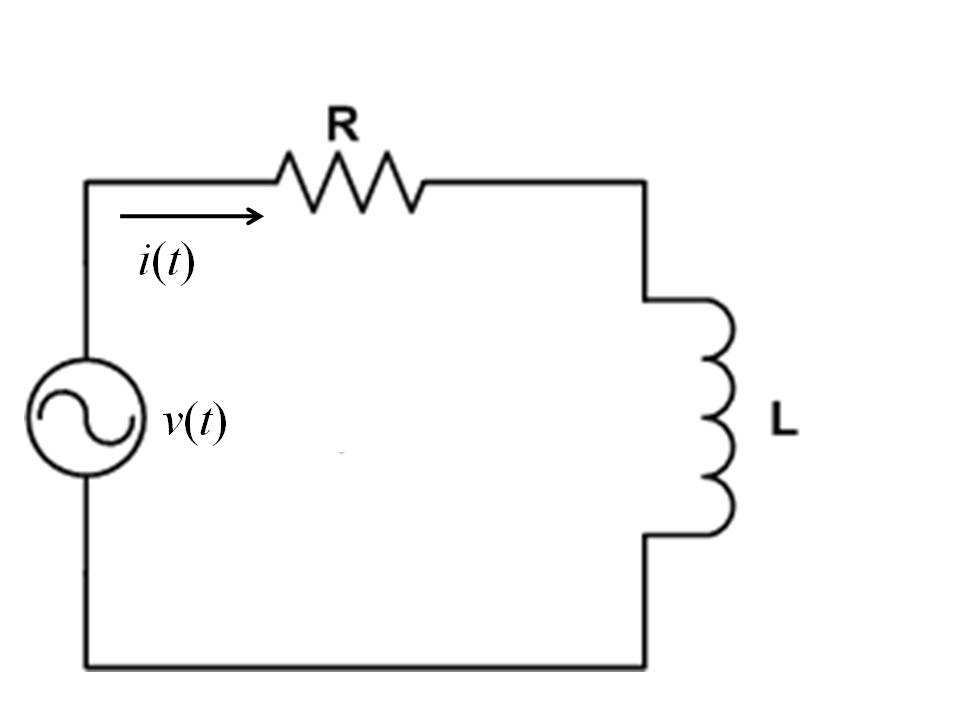
\includegraphics[width=7cm]{RL_circuit}

Using Ohm's Law and Kirchoff's Law it can be shown that $$L\frac{dI}{dt}+RI=V(t)$$  Suppose that the $RL$ circuit above has a resistance of $6$ $  \Omega$ and an inductance of $3$ H.  If a generator produces a variable voltage 
of $V(t)=9\sin{t}$ and the initial current is $I(0) = 2$ A,  find $I(t)$.

Hint: Recall to solve an integral of the form $\int e^x \sin{x} \,dx$, use integration by parts twice.

\includegraphics[scale=0.5]{start.pdf}
{{$I(t)=-\frac{3}{5}\cos{t}+\frac{6}{5}\sin{t}+\frac{13}{5}e^{-2t}$}}
\includegraphics[scale=0.5]{end.pdf}





\end{enumerate}

\end{document}